\documentclass[../main.tex]{subfiles}
\hbadness=1000000
\vbadness=1000000
\begin{document}
\section{Introduction}

In this chapter, we cover our work with an ongoing collaboration with a research group 
in the  C3N (Centre for Cognitive and Computational Neuroscience, Universidad Complutense de Madrid, Spain).
This collaboration arises from the proposal to design a clinical protocol aimed at preventing the development of severe diseases such as Alzheimer's disease.
Our contribution to this proposal is the development of a computational model to apply the proposed method and be able to make predictions about its potential application in patients.
Specifically, this chapter encompasses the initial steps in developing this model, where we have established a methodology to build upon.

As a result of this collaboration, we have published a paper entitled \textit{Understanding the Effects of Cortical Gyrification in tACS: Insights from Experiments and Computational Models} \citep{cabrera-alvarez_understanding_2023}, which a big part of the contests presented here, are summarized there.

\subsection{Resting-state functional networks}
Understanding the intricate relationship between the structure and function of the human brain is a fundamental pursuit in the field of Neuroscience.
In the absence of external stimulation, our mental states fluctuate as the brain moves from one pattern of activity to another.
Although these fluctuations are typically considered nuisances in cognitive task studies, they possess inherent structure and valuable information.
Through functional magnetic resonance imaging (fMRI) and other neurophysiological imaging techniques, it has been observed that spontaneous brain activity can be decomposed into networks of interconnected brain regions, the so-called Resting-State Networks (RSN).
Some of these RSNs include sensorimotor, visual, and attentional networks that have been identified in the absence of specific tasks \citep{seitzman_state_2019}.
\begin{figure}[!htb]
    \centering
    % 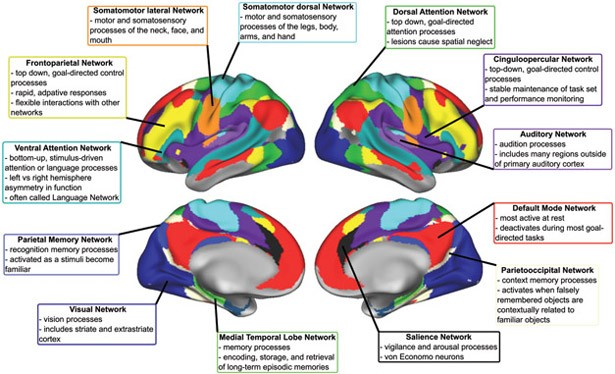
\includegraphics[width=\textwidth]{chapter3/figures/RSNs.jpg}
    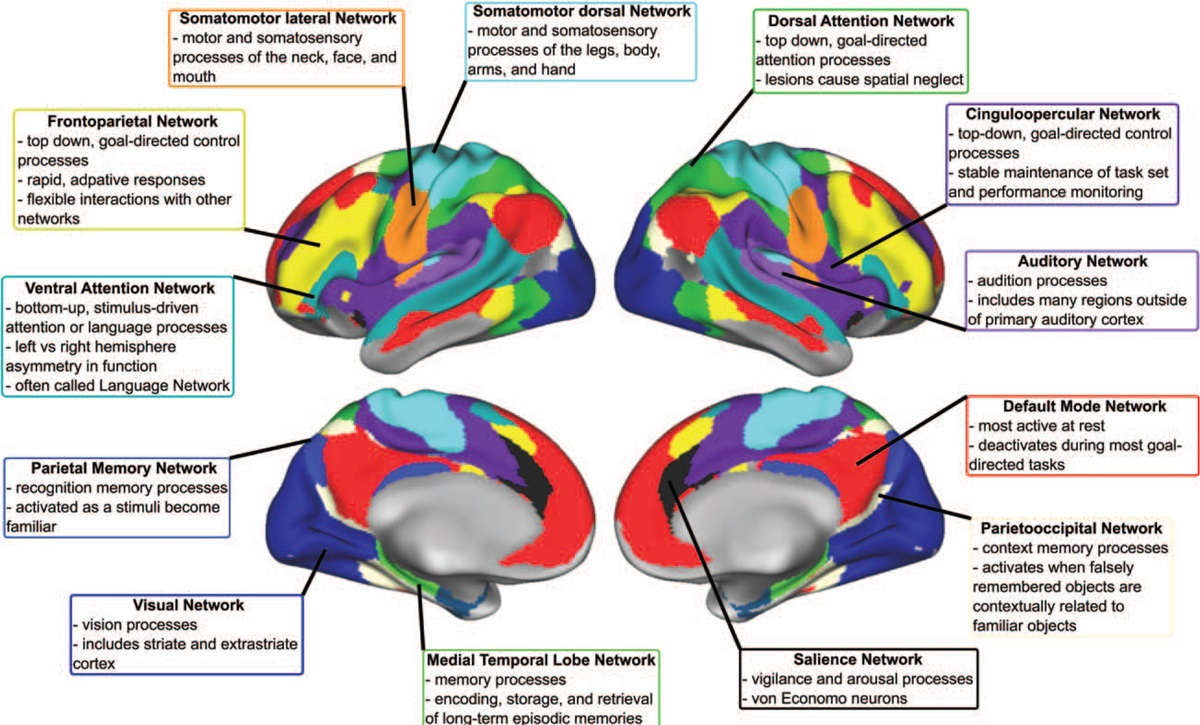
\includegraphics[width=\textwidth]{chapter3/figures/RSN_.jpeg}
    \caption{\textbf{Resting-state networks}.
    Different resting-state networks identified and under research currently. 
    Figure original from \citep{seitzman_state_2019}.}
    \label{fig:RSNs}
\end{figure}
A distinct Default Mode Network (DMN) has been recognized, which exhibits higher activity during rest compared to various task conditions, and has been associated with daydreaming, free association, stream of consciousness, or inner rehearsal. Upwards of 90\% of the energy consumed by the brain is used to support the DMN \citep{raichle2007default,deco_key_2009}.
Figure \ref{fig:RSNs} shows a full list of all the RSNs identified.

The dynamics and characteristics of these functional networks are influenced by both the underlying anatomical connectivity and local neuronal dynamics, resulting in spatio-temporal patterns and oscillations at different time scales.
Understanding the origins and mechanisms of these spontaneous functional connectivity patterns is crucial for comprehending the brain's cognitive processes and its ability to regulate mental states.
Consequently, gaining deeper insights into these dynamics requires the application of theoretical models and numerical simulations of resting-state activity.

Resting-state models leverage recent advances in the tracking of white fiber tracts using noninvasive techniques such as diffusion tensor imaging (DTI) or diffusion spectrum imaging (DSI) in humans \citep{cabral_role_2011}.
By integrating realistic neuroanatomical long-range connections between brain areas with local dynamics of the models, such as Kuramoto oscillators \citep{cabral_role_2011}, neural masses \citep{deco_key_2009, honey_network_2007}, or explicitly modeled neurons \citep{deco_ongoing_2012, nakagawa_how_2014}, dynamical cortical models for the human cortex can be constructed.

Simulated activity patterns within these interacting networks have successfully replicated resting-state dynamics.
For instance, models employing various local dynamics, such as chaotic oscillators \citep{honey_network_2007} or Wilson-Cowan oscillators \citep{deco_key_2009}, have been able to reproduce anticorrelated functional networks observed in the cortex.
These modelling approaches provide valuable tools for studying and comprehending the complex dynamics of resting-state functional connectivity patterns.
% Figure \ref{fig:whole-brain-model} shows schematically the process to build this network models. 

% \begin{figure}
%     \centering
%     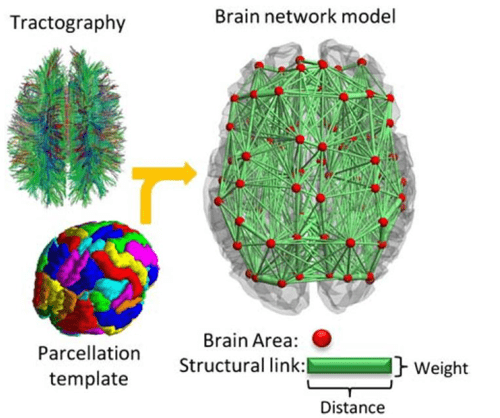
\includegraphics[width=0.5\textwidth]{chapter3/figures/Networks.png}
%     \caption{The spatiotemporal structure of the brain network model.
%     Links are weighted in proportion to the number of white matter fibre tracts and time delays are scaled by the distance between areas.
%     Figure originally from \citep{cabral2017functional}.}
%     \label{fig:whole-brain-model}
% \end{figure}
% \textcolor{blue}{Aquí me gustaría añadir una imagen de un cerebro con diferentes nodos conectados entre sí para que se visualice bien cómo son este tipo de modelos}

\subsection{The role of alpha rhythm}
The alpha rhythm (8-12 Hz) stands out as the most prominent in wakeful (resting-state) magneto/electro-encephalography (M/EEG) recordings \citep{britton_electroencephalography_2016}.
First described in 1929 by Hans Berger \citep{berger_uber_1934}, the alpha rhythm has been associated with cognitive processes such as attention \citep{klimesch2012alpha}, perception \citep{zhou2021alpha,peng2015subjective}, memory \citep{klimesch1997eeg,halgren2019generation}, and aging \citep{knyazeva2018aging}, among others \citep{shaw2003brain}.
When an individual is awake but in a relaxed state with closed eyes, such as during meditation, alpha waves become more pronounced \citep{lomas_systematic_2015}.
This phenomenon has been linked to alpha oscillations with states of decreased cognitive arousal (being awaken) and increased introspection.
Other studies have suggested that alpha band activity plays a crucial role in regulating attentional processes \citep{klimesch_induced_1998, sauseng_shift_2005, bollimunta_neuronal_2011,compton_task_2014}.
When engaged in a task that requires focused attention, the amplitude of alpha waves tends to decrease in the brain region involved in processing that specific task.
This phenomenon is known as alpha suppression and is believed to reflect the inhibition of irrelevant sensory information, allowing individuals to concentrate on the task at hand \citep{compton_task_2014,poland_reduced_2021,clements_dynamics_2022}.

Over the years, the role of the alpha rhythm has been subject to debate.
Initially, its attenuation upon eye-opening and in the presence of visual stimuli led to the notion that alpha oscillations functioned as an 'idling' rhythm, with its amplitude reflecting cortical inhibition \citep{Cliodhna2022}.
However, subsequent research demonstrated that alpha amplitude increases with working memory load and task difficulty \citep{jensen2002oscillations}, and large-scale alpha synchrony has been found to be enhanced within fronto-parietal networks during cognitive tasks \citep{Sadaghiani14305}.
Consequently, it has been proposed that alpha rhythm actively participates in brain functioning \citep{palva2007new}, directly influencing internal representations, mental imagery \citep{cooper2003paradox}, short-term and working memory \citep{klimesch2007eeg}, and top-down modulation \citep{von2000top}.
Furthermore, according to the inhibition-timing hypothesis \citep{klimesch2007eeg}, alpha may play an active role in information processing.

\subsubsection{Abnormalities in the alpha band}
Abnormal behavior within the alpha band has been the subject of considerable research and investigation \citep{arns_effects_2012,locatelli_eeg_1998,adler_eeg_2003,jeong_eeg_2004,uhlhaas_neural_2006,stroganova1999eeg}.
Deviations from normal alpha oscillations have been observed in various neurological and psychiatric disorders, providing valuable insights into the underlying brain dysfunctions.
One common abnormality is excessive alpha power or increased alpha activity.
This abnormality has been associated with conditions such as major depressive disorder, anxiety disorders, and attention deficit hyperactivity disorder (ADHD) \citep{arns_effects_2012}.
It may reflect an imbalance in cortical excitability, leading to difficulties in attention regulation, emotional processing, and cognitive control.
Similarly, abnormalities in reduced alpha power or alpha suppression have also been observed in several disorders.
For instance, individuals with schizophrenia often exhibit decreased alpha suppression during cognitive tasks, suggesting impairments in filtering irrelevant information and maintaining focused attention \citep{arns_effects_2012}.
Reduced power and synchronisation of alpha oscillations has also been consistently associated with neurodegenerative dementias, especially Alzheimer's disease (AD), particularly in posterior brain regions, which could be indicative of disrupted neural network connectivity and cognitive decline \citep{locatelli_eeg_1998,adler_eeg_2003,jeong_eeg_2004,uhlhaas_neural_2006}.
Disrupted alpha coherence, has been observed in individuals with autism spectrum disorders, indicating altered communication and integration between brain regions involved in social cognition and information processing \citep{stroganova1999eeg}.

Additionally, an excess level of synchrony could be a biomarker of disease. 
In AD, the accumulation of Amyloid-$\beta$ in the extracellular space generates an excitation-inhibition imbalance that makes the network to become hyperactive \citep{kazim2021neuronal}.
This high high level of activity is thought to be linked to the hyper-synchronization observed between fronto-parietal areas (specifically between \textit{Anterior Cingulate Cortex} and \textit{Precuneus}) at early stages: in cognitively intact AD relatives \citep{ramirez2021functional}, patients with subjective cognitive decline \citep{hafkemeijer2013increased, lopez2017functional} and early stages of mild cognitive impairment (MCI) \citep{lopez_alpha-band_2014}.
Therefore, reducing the hyper-synchrony between those brain areas, at the early stages, could be a potential therapeutic protocol to slow down the evolution of Alzheimer's disease.
\clearpage
\subsection{Transcranial alternating current stimulation}
Transcranial alternating current stimulation (tACS) is a promising non-invasive tool for modulating brain oscillations.
It consists on stimulating the brain with external electrical currents that are likely to influence the oscillatory activity of the neurons at specific frequencies.
Like other brain stimulation techniques, tACs has the potential to enhance our understanding of brain function by establishing causal relationships between brain activity, cognition, and behavior \citep{herrmann2013transcranial,dayan2013noninvasive,polania2018studying}.

The underlying mechanism of tACS involves the delivery of weak electrical currents through the skull, which modifies the polarization of cellular membranes and alters the thresholds for neural activation \citep{reato2013effects,liu2018immediate}.
This effect can improve the synchronization of neural activity by adjusting the timing of neural activation to align with the rhythm of the stimulation, the so-called entrainment \citep{helfrich2014entrainment, vogeti2022entrainment, liu2018immediate}.
Furthermore, recent studies have suggested that tACs may also affect neural plasticity by inducing long-term potentiation and depression \citep{schwab2021spike, jeong2021modulation}.

tACS has shown potential in addressing the reduction of alpha power observed in various disorders.
Some studies have investigated the application of tACS at the individual alpha frequency (IAF, the peak frequency) to enhance alpha oscillations \citep{zaehle_transcranial_2010, helfrich2014entrainment, kasten2019integrating, zarubin_transient_2020}.
\begin{figure}[!htb]
    \centering
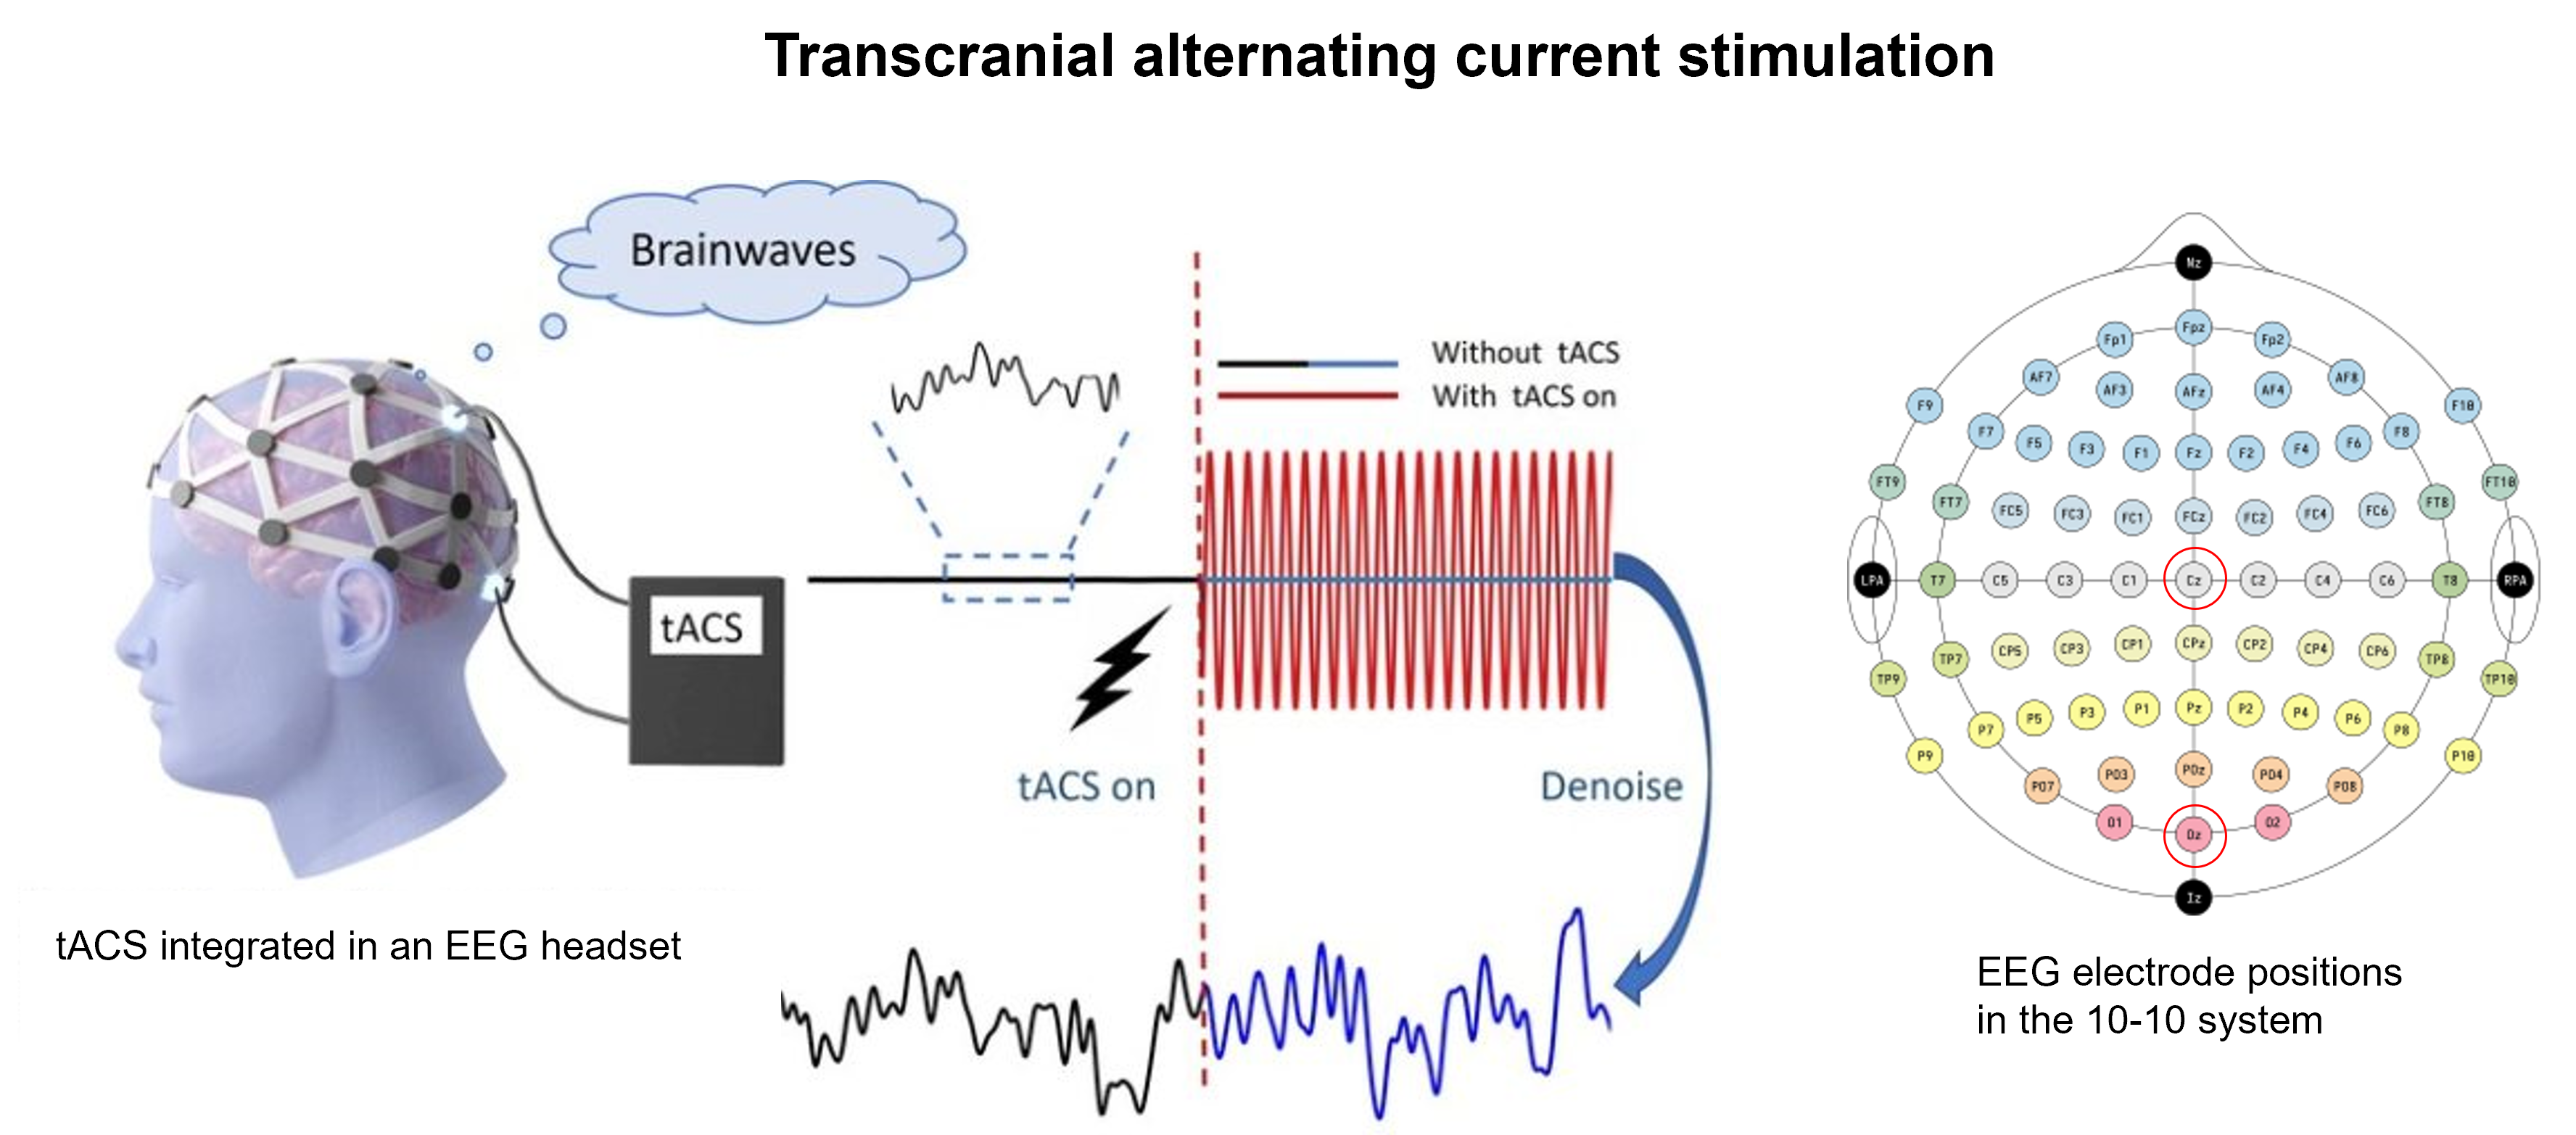
\includegraphics[width=\textwidth]{chapter3/figures/tacs_schematics.png}
    \caption{\textbf{Transcranial alteranting current stimulation (tACS) procedure}.
    The stimulation is integrated into the EEG headseat.
    The EEG electrode positions in the 10-10 system labelled with the modified combinatorial nomenclature is represented in the right. 
    Circled nodes indicate Cz and Oz electrodes, midline central and midline occipital, respectively; that represents the regions where tACS is applied.
    Figure adapted from \citep{9743292} and \citep{EEGlabels}.}
    \label{fig:EEG}
\end{figure}
For instance, in some experiments, this enhancement resulted in an increase of 14\% of spectral power across subjects \citep{zaehle_transcranial_2010}.
In these experiments, IAF-tACS stimulation is administered to parieto-occipital regions to synchronize with the dominant posterior alpha rhythm.
However, the results of these studies are inconsistent, both in terms of the effectiveness of the stimulation and the locations where the effects are observed.
Several factors can influence the outcomes of tACS, including the choice of electrode placements, current intensity, targeted brain regions, skull conductivity, head positioning, cortical structure, and the orientation of the neurons \citep{datta2012inter,guerra2020variability,huang2018roast,kasten_integrating_2019}.

The administered currents in humans typically do not exceed 1-2 mA peak intensity \citep{liu2018immediate,zaehle_transcranial_2010, helfrich2014entrainment, kasten2019integrating, zarubin_transient_2020}.
Intracranial measurements conducted in epilepsy patients have revealed that the amplitude of the electrical fields reaching the brain with 1 mA peak intensity currents is generally below 0.5 V/m \citep{liu2018immediate}.
Despite these relatively modest field strengths, they appear to be sufficent for enhancing alpha oscillations in specific brain regions, as evidenced by experiments where the maximum applied current was 1 mA. 
Conversely, investigations in rodent models, where applied fields can be tenfold stronger or even more (6.8 $\pm$ 2.3), have elucidated the capacity of tACS to elicit physiological effects on spike timing, LFP oscillations, and the cessation of seizure patterns \citep{liu2018immediate}.

% \textcolor{red}{Dudoso: The application of sinusoidal electrical currents over the scalp influences the excitability of the targeted neuronal groups by subthreshold polarizing inputs \citep{radman2009role, de_ridder_noninvasive_2017}.
% The orientation of the electric field with respect to cell bodies' axis contributes to the magnitude and effect, either depolarizing or hyperpolarizing of the neurons' membrane potential.}
% \textcolor{blue}{Aquí me gustaría poner una imagen del protcolo de tACS junto con una imagen donde se vean los nodos del casco y su nombre. Puesto que nos referimos todo el rato al protocolo OzCz}
% \textcolor{blue}{Vale, lo que me refería era el caso de EEG, que he mezclado cosas. Tengo que darle una pensada a como meterlo (si hacerlo)}

\subsection{Computational models of electric field propagation}
Computational modelling has emerged as a valuable and indispensable tool to investigate the mechanistic effects of electrical stimulation on the brain.
Two types of models stand out in this field of research: \textbf{current propagation} models and \textbf{neural activation} models.
\textbf{Current propagation} models aim to analyze, predict and regulate the electric fields generated within the brain as a result of applied stimulation.
These models consider various factors such as the specific montages used for stimulation, the shape of different head tissues, and their impact on electric fields \citep{miranda2006modeling, holdefer2006predicted, russell2014gender,forssell2021effect, huang2017measurements}. 
In contrast, \textbf{neural activation} models offer a detailed understanding of how electric fields generated by stimulation affect the activation of neural tissue across different levels of analysis, ranging from individual cells to the entire brain. These models provide a comprehensive explanation of the effects of stimulation by simulating the interaction between electrical fields and neural activity \citep{merlet_oscillatory_2013, deco2019awakening, aberra2020simulation,  meier_virtual_2021, tran2022effects, wang2023responses}.
These two models can be integrated into a large-scale brain networks models allowing for \textit{in-silico} stimulation and investigation of stimulation effects \citep{merlet_oscillatory_2013}.

To ensure the accuracy and validity of these network models, they are calibrated and validated using empirical data, functional and structural connectivity, aiming to closely replicate the phenomenon being studied.
The combination of empirical data with the computational framework allows us to strengthen our understanding of the underlying mechanisms of electrical stimulation and its impact on brain function.
This interdisciplinary approach provides valuable insights into the complex interactions between electrical stimulation and the brain.
% \clearpage
\subsection{Objectives}
The objective of this work is to develop a tACS protocol with the potential to become a clinical tool aplicable to Alzheimer's disease in individuals with Mild Cognitive Impairment. 
To achieve this, we propose a theoretical-experimental project, with the aim of developing a methodology to generate personalized resting-state network models for each subject.
This personalization is achieved through the use of structural connectivity matrices (tracts and their lengths) and functional connectivity matrices.
Once this is done, the experiment would be structured in two steps.
First, determine an increase in the alpha peak for each subject using tACS.
Following previous protocols, the intensity level of stimulation would be determined by the moment in which the patient feels the presence of a sensation \citep{zaehle_transcranial_2010}. 
This increase would be replicated with the computational model to establish a relationship between the experimental tACS intensity and the model tACS intensity.
Second, we would activate the desynchronization protocol by stimulating frontal or parietal regions, as no differences in stimulation effects are expected between these areas.
In this protocol, we will apply tACS using the intensity that yields the maximum power (determined in the previous step) and sweep the frequency around the IAF until we find the value that leads to the maximum desynchrony between the precuneus and the anterior cingulate cortex.

In this chapter, we develop a customized resting-state network model using spiking neurons and evaluate under which conditions the application of tACS leads to an increase in the power of alpha-band population activity.
\clearpage
\end{document}